\documentclass{article}
\usepackage{graphicx}
\usepackage{tikz}
\usepackage[export]{adjustbox}
\usetikzlibrary{shapes.geometric, arrows, positioning, fit}

\title{Assignment 3\\ `Whisper'\\ System Design}
\author{
    Joakim Tollefsen Johannesen\\
    \texttt{joakimtj@hiof.no}
    \and
    Niklas Berby\\
    \texttt{niklab@hiof.no}
}
\date{2024}

\begin{document}
\maketitle
\section{Technical Structure}
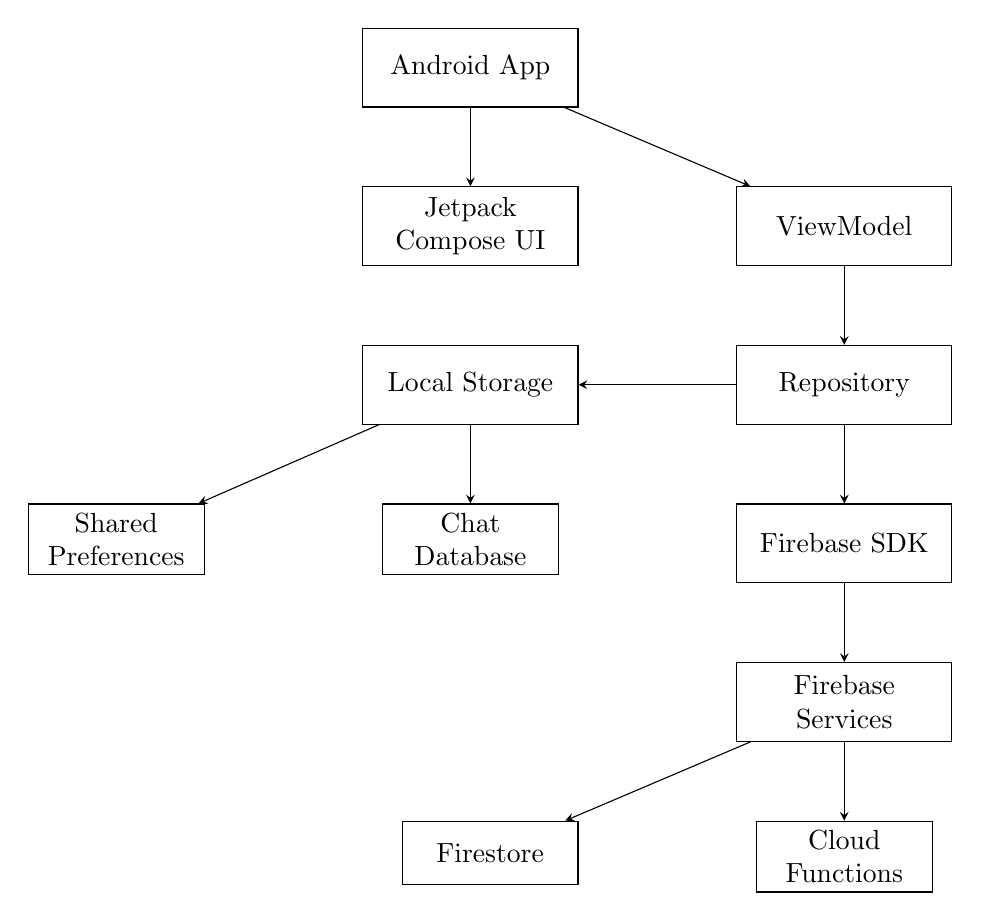
\begin{tikzpicture}[
    node distance = 1cm and 2cm,
    box/.style = {rectangle, draw, text width=2.5cm, text centered, minimum height=1cm},
    smallbox/.style = {rectangle, draw, text width=2cm, text centered, minimum height=0.8cm},
    arrow/.style = {->, >=stealth}
]

% Define nodes
\node[box] (app) {Android App};
\node[box, below=of app] (ui) {Jetpack Compose UI};
\node[box, right=of ui] (viewmodel) {ViewModel};
\node[box, below=of viewmodel] (repository) {Repository};
\node[box, below=of repository] (firebase) {Firebase SDK};
\node[box, below=of firebase] (services) {Firebase Services};
\node[smallbox, below left=of services] (firestore) {Firestore};
\node[smallbox, below=of services] (functions) {Cloud Functions};
\node[box, left=of repository] (local) {Local Storage};
\node[smallbox, below left=of local] (prefs) {Shared Preferences};
\node[smallbox, below=of local] (room) {Chat Database};

% Draw arrows
\draw[arrow] (app) -- (ui);
\draw[arrow] (app) -- (viewmodel);
\draw[arrow] (viewmodel) -- (repository);
\draw[arrow] (repository) -- (firebase);
\draw[arrow] (firebase) -- (services);
\draw[arrow] (services) -- (firestore);
\draw[arrow] (services) -- (functions);
\draw[arrow] (repository) -- (local);
\draw[arrow] (local) -- (prefs);
\draw[arrow] (local) -- (room);

\end{tikzpicture}

\newpage 
\begin{itemize}
    \item Data storage and management:
    \begin{itemize}
        \item Firebase Firestore to store chats, messages and user data.
        \item Firestore will handle chat and message synchronization.
        \item E.g., room exipration.
    \end{itemize}
    \item User management:
    \begin{itemize}
        \item There is no user authentication planned due to the anonymized nature of the app.
        \item Most relevant user data (preferences as such) will be stored locally.
    \end{itemize}
\end{itemize}

\section{Navigation}

Below is a graph representation of the app's navigation. The screens are unlikely to change much from the project proposal outside of changes made to comport with Material Design principles.

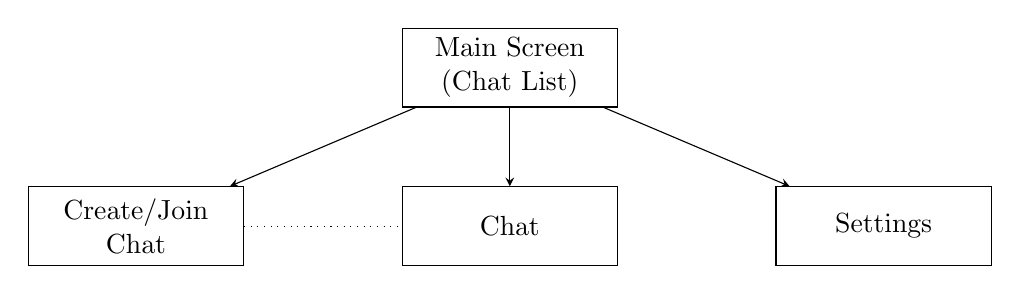
\begin{tikzpicture}[
    node distance = 1cm and 2cm,
    box/.style = {rectangle, draw, text width=2.5cm, text centered, minimum height=1cm},
    smallbox/.style = {rectangle, draw, text width=2cm, text centered, minimum height=0.8cm},
    arrow/.style = {->, >=stealth}
]

% Define nodes
\node[box] (main) {Main Screen (Chat List)};
\node[box, below=of main] (chat) {Chat};
\node[box, below right=of main] (settings) {Settings};
\node[box, below left=of main] (joinchat) {Create/Join Chat};


% Draw arrows
\draw[arrow] (main) -- (chat);
\draw[arrow] (main) -- (settings);
\draw[arrow] (main) -- (joinchat);
\draw[dotted] (joinchat) -- (chat);


\end{tikzpicture}

The dotted lines represent navigation to the chat that has been joined/created. \\

After some consideration, we've decided that we will join the Create and Join screens together.

The primary screens we have planned are shown in the images below.

\begin{center}
    \fbox{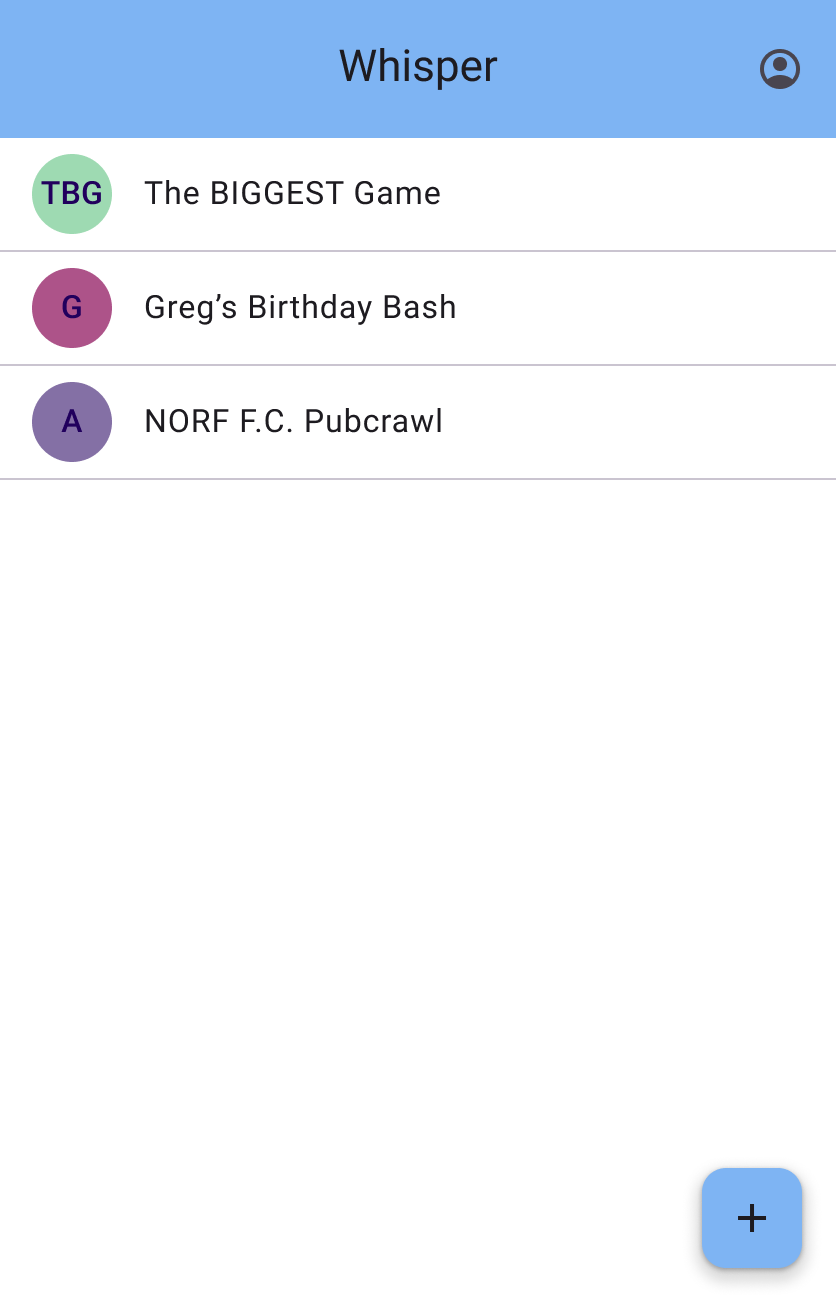
\includegraphics[scale=0.25]{imgs/main.png}}
    \fbox{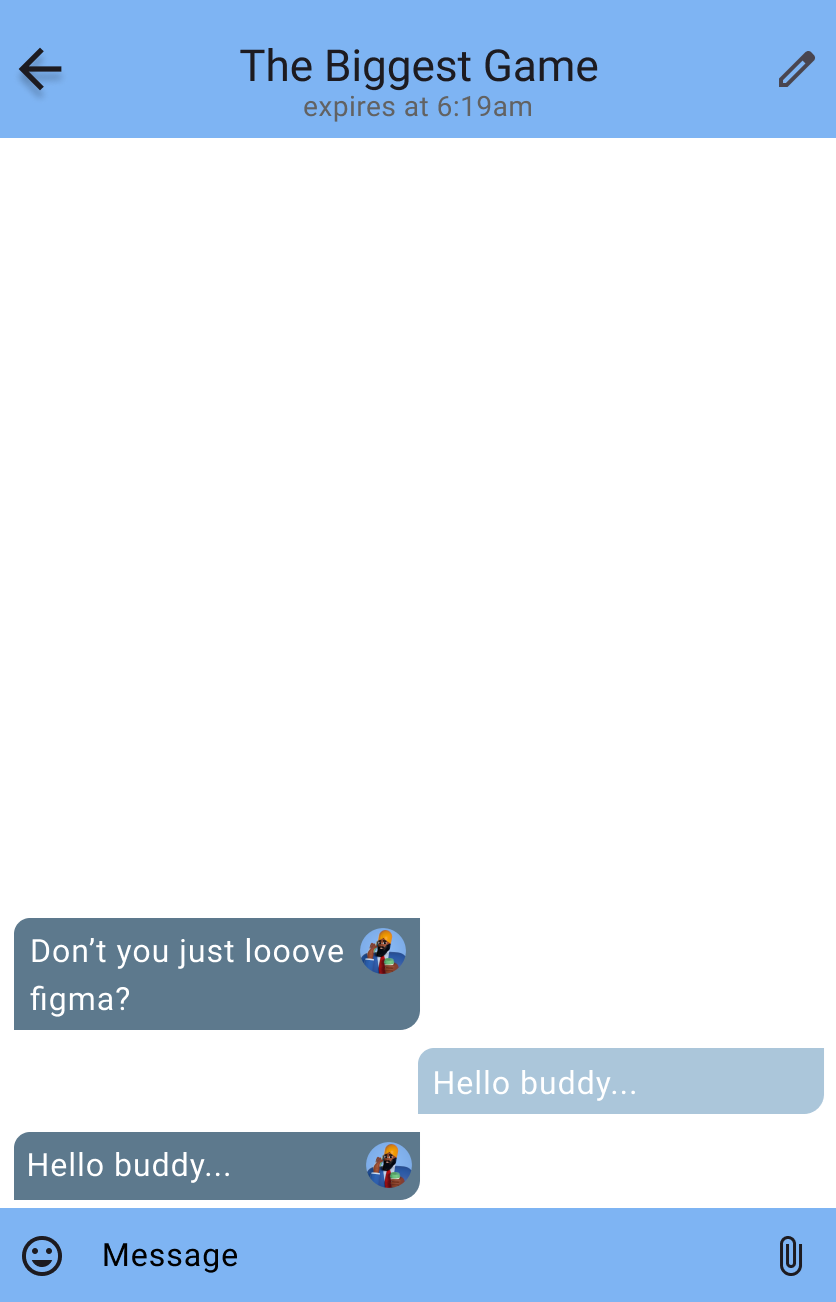
\includegraphics[scale=0.25]{imgs/chat.png}}
    
\end{center}

\begin{center}
    \fbox{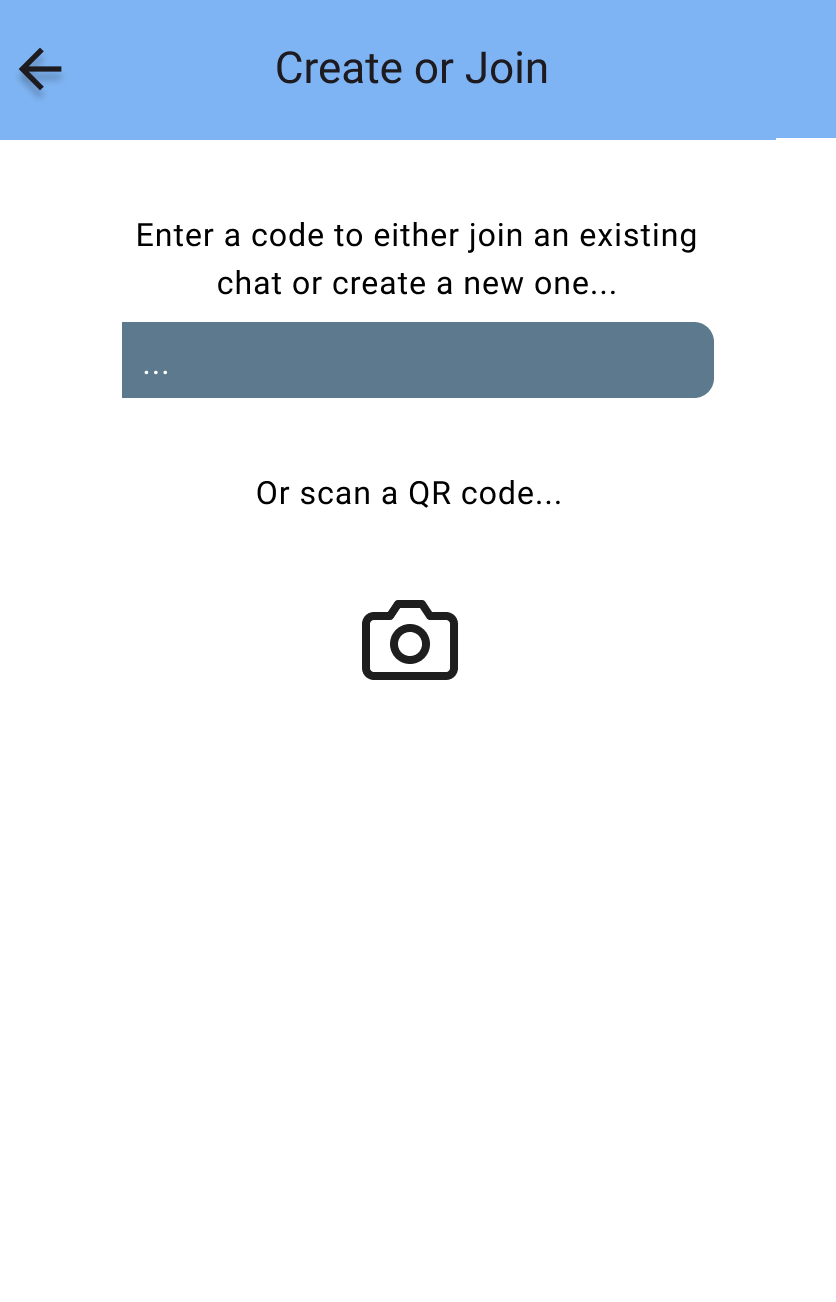
\includegraphics[scale=0.25]{imgs/createorjoin.png}}
    \fbox{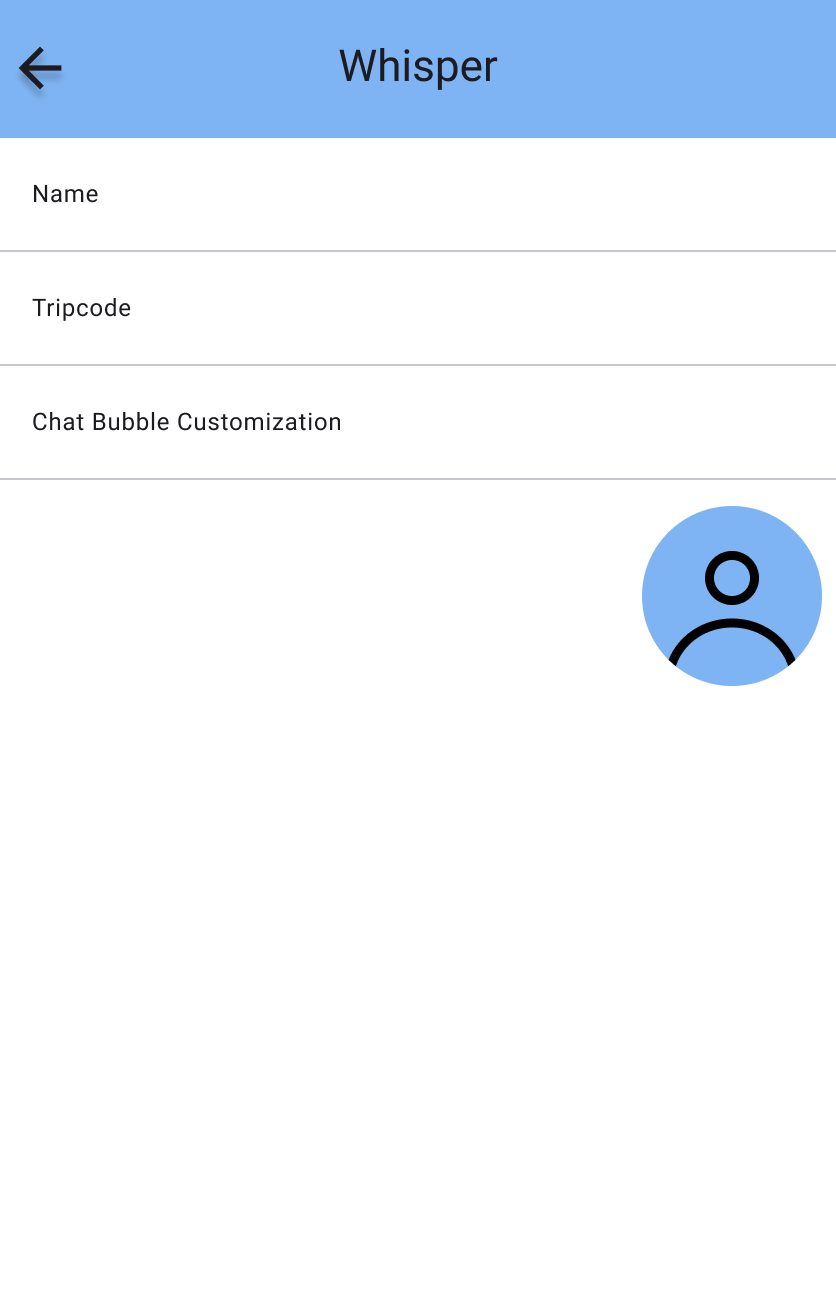
\includegraphics[scale=0.25]{imgs/profile.png}}
\end{center}

\section{Resources}

We plan to source most art assets externally if we deviate from this we will, of course, document it. It's a little difficult to make this decision right now. But we do know that the following will be sourced externally: 
\begin{enumerate}
    \item Material Design symbols for common actions.
    \item Sound effects (if implemented). E.g. push notifications.
\end{enumerate}
\end{document}